\section{Experiments}

In this section, we aim to address the following research question: "How does the state-of-the-art T5-PICARD method perform on the SEOSS Dataset compared to SQLNet and RatSQL, and can general-purpose language models be effectively employed to solve the text-to-SQL problem?" To answer this question, we conduct experiments using the T5-PICARD approach, which has been recently proposed for the SPIDER challenge, and compare its performance to SQLNet and RatSQL, as documented in the SEOSS-Queries research paper\cite{TOMOVA2022108211}. The results of these experiments, presented in the subsequent section, demonstrate the capabilities of the T5-PICARD method in tackling the SPIDER task using the SEOSS Dataset.

Furthermore, considering the recent advancements in large language models and the availability of the ChatGPT APIs, we explore the performance of GPT models on this task. We conduct experiments using the SPIDER and SEOSS datasets and compare the findings to those obtained from earlier experiments with SQLNet and RatSQL. The insights from these experiments, discussed in the following section, shed light on the potential of modern large-scale language models, such as GPT, in addressing the SPIDER task and further contribute to answering our research question. This investigation also helps determine if general-purpose language models can effectively solve the text-to-SQL problem.

\subsection{Limitations}

Our experiment faced several limitations, primarily due to the extensive computational resources required when leveraging the T5 model. For our experiment, we used a single Nvidia RTX 3070 16GB GPU with 20GB Memory, which constrained us to smaller models with tighter restrictions. Despite these limitations, we managed to achieve admirable results. Utilizing a larger T5 model could have led to even higher scores. As a result, investing in a more powerful GPU for our experiment should be considered to capitalize on our model's potential fully.
In addition, during the ChatGPT experiment, cost constraints limited our ability to experiment with GPT-4.0, as its usage cost is approximately 30 times higher than that of GPT-3.5-turbo. We had to experiment with different methods to find the best prompt for ChatGPT to force him to act as a text-to-SQL agent, but this led to wasting money.

\begin{table}[H]
    \centering
    \begin{tabular}{|l|l|}
        \hline \textbf{Model} & \textbf{Usage}      \\
        \hline GPT-4          & \$0.06 / 1K tokens  \\
        \hline GPT-3.5-turbo  & \$0.002 / 1K tokens \\
        \hline
    \end{tabular}
    \caption{Cost comparison between GPT-4 and GPT-3.5-turbo}
    \label{tab:cost_comparison}
\end{table}

\subsection{SEOSS evaluation with T5 PICARD}

\begin{figure}[H]
    \begin{AIbox}{Additional Materials}
        \parbox{1\textwidth}{
            The code and evaluated experiment results are detailed in the provided GitHub repository and the CD attached to this thesis.
        }
    \end{AIbox}
\end{figure}

After studying the SEOSS dataset, we decided to experiment with the PICARD model\ref{picard} to evaluate its performance against that of SQLNet and RatSQL. We decided to use the T5-Base and T5-Large models for our experiment, as they are smaller than the T5-3B and T5-11B models used by most state-of-the-art studies. To ensure a fair comparison between the models, we used two beam sizes of 2 and 4 and the same evaluation metrics as SEOSS-SQLNet and SEOSS-RatSQL, which is "exact matching accuracy". We wanted to see if the PICARD model could achieve similar results to those of SQLNet and RatSQL, so we conducted our experiment with our findings. The results of our experiment are discussed in the following section and can be used to compare the performance of the PICARD model to the models used in the SEOSS study.
\footnote[1]{Link to the Github Page: \url{https://github.com/yazdipour/text-to-sql-seoss-t5}}

\begin{table}[!ht]
    \centering
    \begin{tabular}{ccccc}
        \hline
        Model    & Picard Mode       & Beams & \textbf{Exact Matching Accuracy} & \textbf{Execution Accuracy} \\ \hline
        T5-base  & lex               & 4     & 0.3071                           & 0.3039                      \\ \hline
        T5-base  & parse with guards & 2     & 0.3297                           & 0.3576                      \\ \hline
        T5-base  & parse with guards & 4     & 0.3286                           & 0.3512                      \\ \hline
        T5-large & lex               & 2     & 0.3672                           & 0.3629                      \\ \hline
        T5-large & parse with guards & 4     & 0.4274                           & 0.4822                      \\ \hline
    \end{tabular}
    \caption{Expermiment Accuracy Results}
    \label{tab:exp-acc-t5}
\end{table}

Table \ref{tab:exp-acc-t5} presents the performance results of various configurations of T5-base and T5-large models in natural language processing tasks, with distinctions based on the utilization of Picard mode (either parse with guards or lex) and the number of beams (2 or 4) employed in the beam search process. Upon comparing the results, it becomes evident that the T5-large model outperforms the T5-base model regarding exact matching and execution accuracy. Additionally, as anticipated, the parse with guards Picard mode demonstrates superior performance compared to the lex Picard mode in both T5 models, leading to the decision to proceed exclusively with the parse with guards mode.

Furthermore, employing four beams in the beam search process, as opposed to two, enhances performance across both models and Picard modes. The T5-large model achieves its highest exact matching accuracy (0.4274) and execution accuracy (0.4822) when utilizing the parse with guards Picard mode in conjunction with four beams. Interestingly, the impact of increasing the beam size is relatively negligible compared to the performance improvement gained from upgrading the model from T5-base to T5-large.

\subsubsection*{F1 Scores}

% add image here pics/ez/F1.svg
\begin{figure}[H]
    \centering
    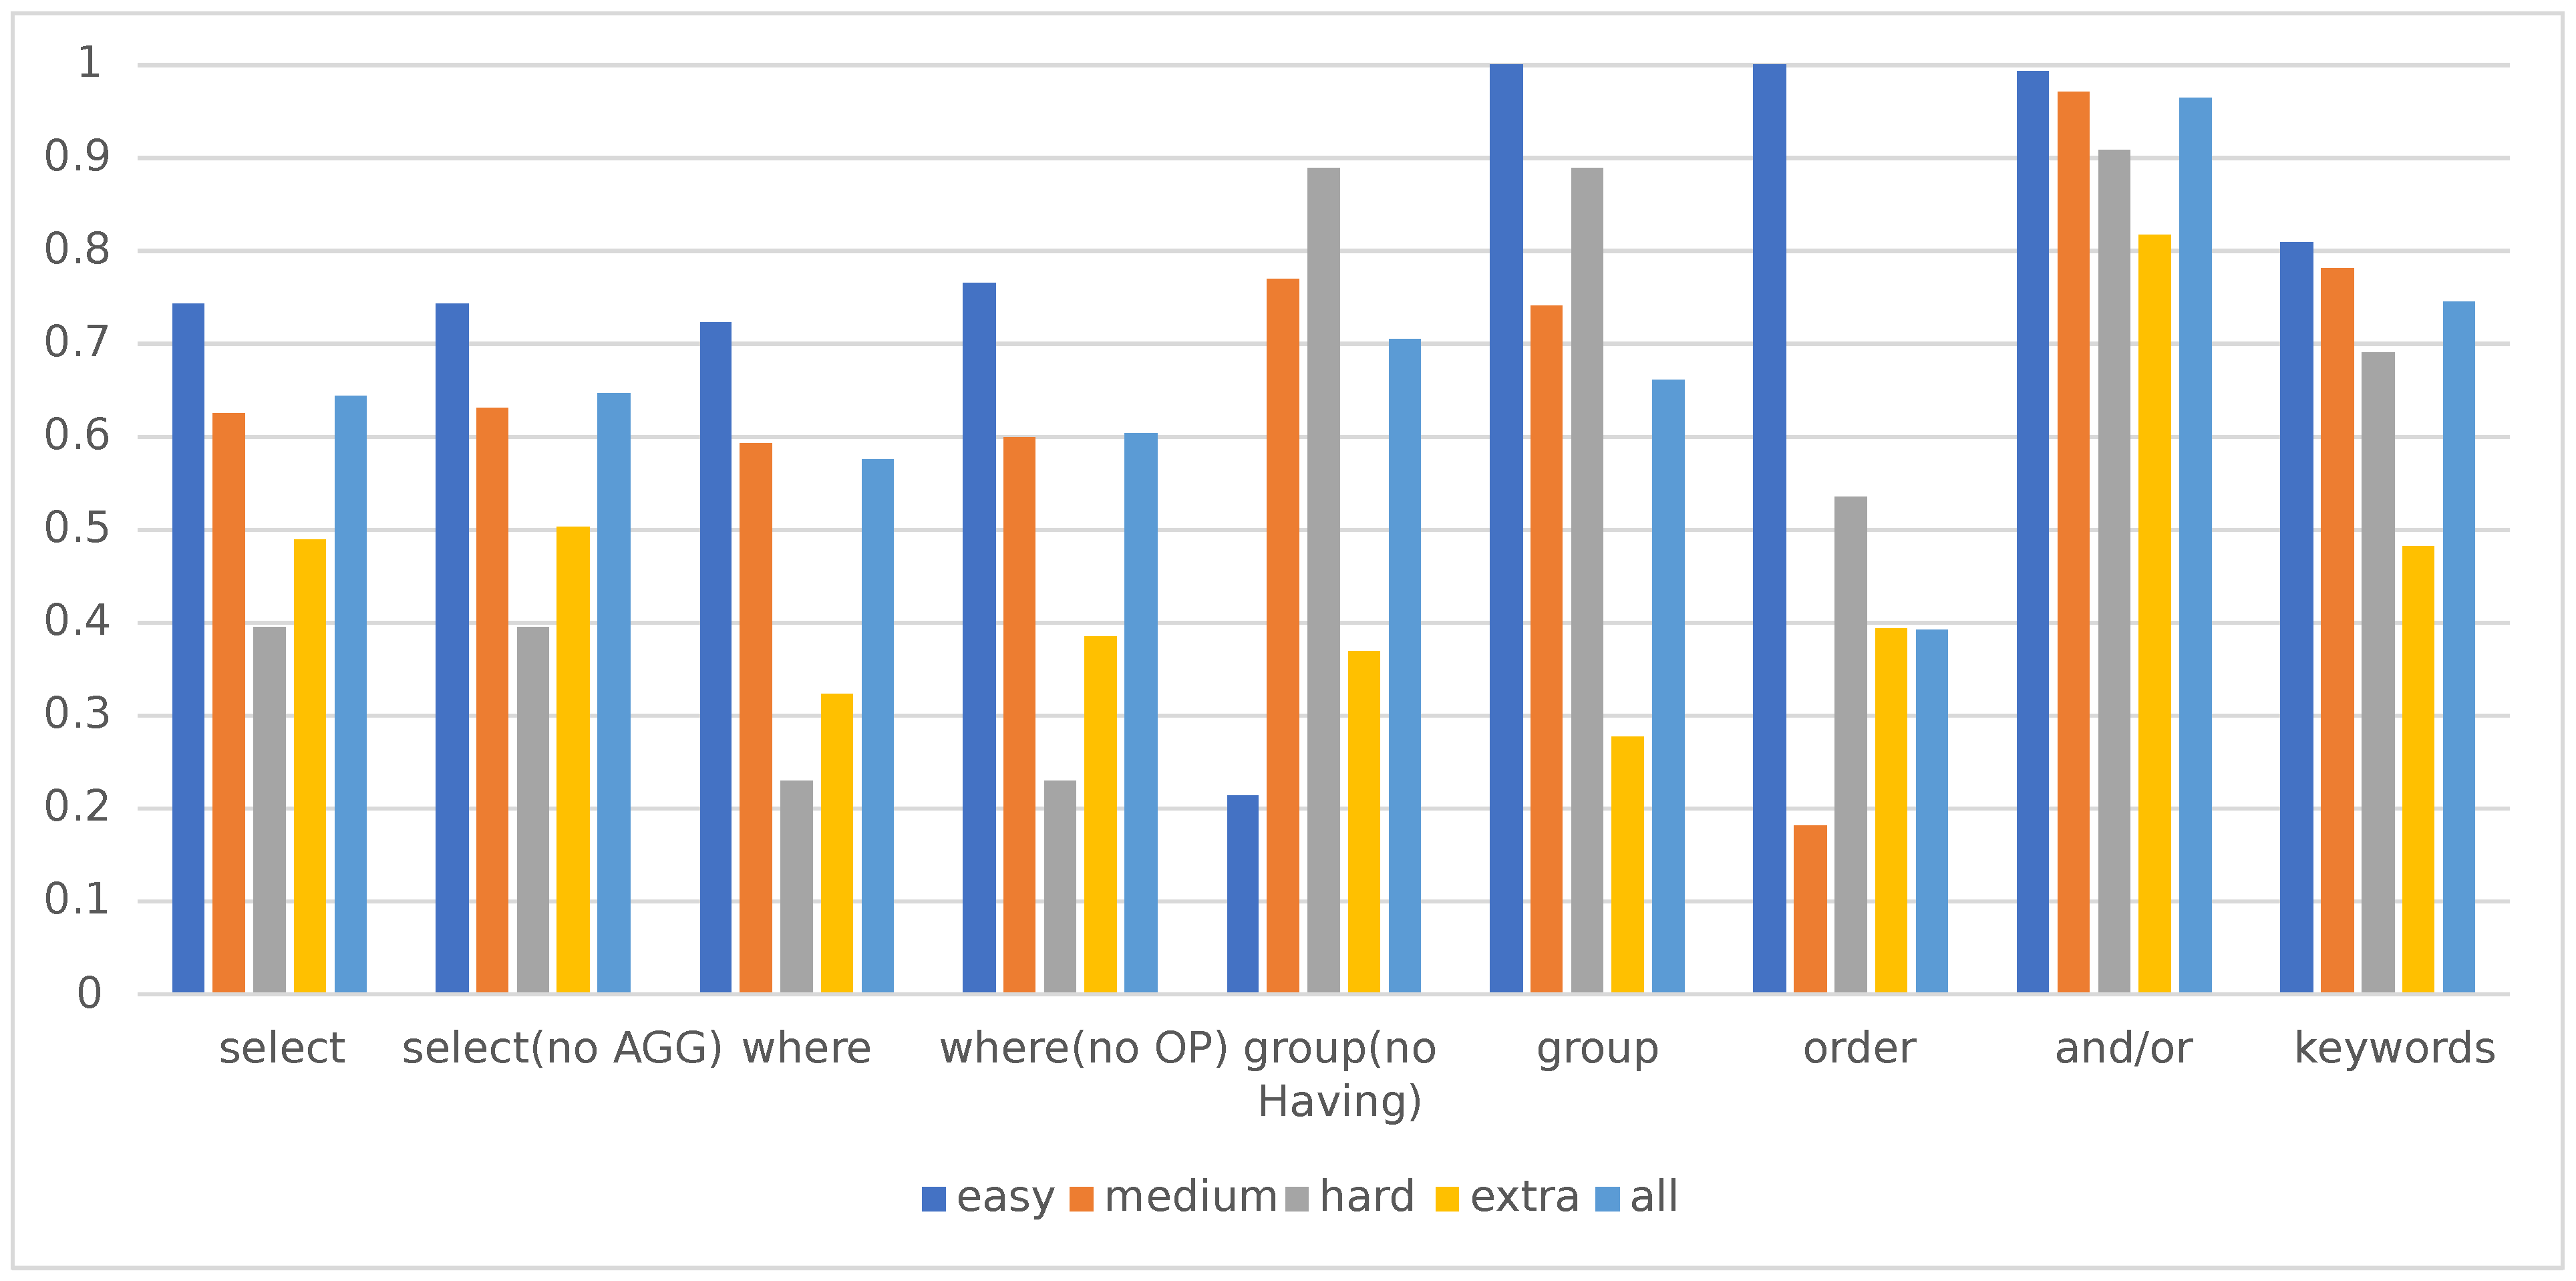
\includegraphics[width=1\textwidth]{pics/ez/F1eps}
    \caption{F1 Scores of Component Matching - PICARD T5-Large 4-Beam}
\end{figure}

Here, we can observe the F1 scores of each SQL Keyword for the PICARD T5-Large 4-Beam experiment on the SEOSS dataset. We can see that PICARD has managed to attain a very impressive F1 score for the SEOSS dataset without even having to be specifically trained for our dataset. This is a very encouraging result and indicates that the model is able to generalize accurately across different domains. Moreover, it is essential to note that the F1 score obtained by the PICARD model was obtained without any additional fine-tuning. This is a testament to the robustness and capability of the model and further highlights its ability to generalize to different datasets.

We experimented with a variety of different parameters, including beam size, modes and model sizes, and spent multiple hours for each evaluation. These experiments have been carefully documented in the Appendix of this thesis, where you can also find them in the project repository.

\clearpage
\subsection{SEOSS evaluation with GPT 3.5 and GPT 4}  

Here we discuss our experience using the ChatGPT API for the Text-to-SQL task on the SEOSS dataset. We will provide a brief overview of the \ac{GPT} architecture and delve into the specifics of ChatGPT, emphasizing its capabilities and potential for addressing this particular challenge.
\subsubsection{GPT Architecture}

Generative Pre-trained Transformers (GPT) \cite{radford2018improving} represent the state-of-the-art in language modeling, being built upon the revolutionary Transformer architecture. This architecture has profoundly influenced the field of natural language processing due to its utilization of self-attention mechanisms. These mechanisms enable the parallel processing of sequences, leading to more efficient training and enhanced performance across a wide range of NLP tasks.

Inherently generative, GPT models are designed to create text based on the context they are given. They are pre-trained on vast quantities of textual data, which enables them to learn the underlying structure and patterns present in natural language. The pre-training phase consists of unsupervised learning using a masked language modeling objective. Following pre-training, GPT models can be fine-tuned for specific tasks, such as translation, summarization, or, as in our example, Text-to-SQL.

Prior to the introduction of GPT-4, OpenAI had developed three earlier GPT versions and had been refining GPT language models over an extended period. The first GPT model, launched in 2018, incorporated 117 million parameters. The next version, GPT-2, was released in 2019 and demonstrated a substantial increase, incorporating 1.5 billion parameters. GPT-3, which currently powers ChatGPT, made its debut in 2020 and operates with 175 billion parameters. OpenAI, however, has chosen not to reveal the number of parameters used in GPT-4 \cite{openai2023gpt4}.

Considering the consistent growth in parameter counts with each successive model, it is logical to assume that the most recent multimodal iteration features a higher number of parameters than its predecessor, GPT-3, which consists of 175 billion parameters. Also, some researchers have speculated that GPT-4 may have as many as 1 trillion parameters or more\cite{bubeck2023sparks}.

\subsubsection{ChatGPT}

\begin{figure}[H]
    \begin{AIbox}{Attention!}
        \parbox{1\textwidth}{
            Please note that the results in this section may be subject to change as ChatGPT continues to improve its system over time.
        }
    \end{AIbox}
\end{figure}


ChatGPT and \ac{LLM} models represent an evolution in language models tailored explicitly for conversational interfaces. These models exhibit a distinct behavior compared to older language models. While previous models operated on a text-in and text-out basis (accepting a prompt string and returning a completion to append to the prompt), GPT-3 and GPT-4 models follow a conversation-in and message-out approach \cite{bubeck2023sparks}. They expect input formatted in a chat-like transcript format and return a completion representing a model-generated message within the chat. This format is designed for multi-turn conversations but can also be effective in non-chat scenarios.
For our experiment with the SEOSS dataset, we utilized the ChatGPT API to submit natural language questions and retrieve generated SQL queries. The API allowed for the seamless integration of ChatGPT into our workflow and provided an efficient and effective means to process the dataset.
Throughout the evaluation, we observed that ChatGPT successfully generated accurate and syntactically correct SQL queries for a wide range of questions. The model excelled at handling complex queries and demonstrated a deep understanding of the underlying database schema.
However, there were instances where ChatGPT generated SQL queries that deviated from the desired output, particularly in edge cases and questions with ambiguous semantics. To mitigate this issue, we employed a combination of custom LLM prompts to ensure the generated queries met the required quality standards.

\subsubsection{ChatGPT Prompting}

\subsubsubsection{Rules}

ChatGPT employs prompts to direct its response generation process \cite{white2023prompt}. 
To maximize the effectiveness of ChatGPT in various applications, it is essential to understand the art of crafting effective prompts. The following guidelines have been established to optimize the performance of ChatGPT in generating accurate, relevant, and context-aware responses:

\begin{enumerate}
    \item \textbf{Give ChatGPT an identity and intended audience}: By assigning a role or identity to ChatGPT (e.g., "You are a text-to-sql assistant, do... or As an assistant, do...") and specifying the target audience, the model can adopt a specific perspective or tone, providing tailored responses to the context.

    \item \textbf{Offer and give specific context}: Including relevant background information or context in the prompt helps the model generate more accurate and meaningful answers, particularly when dealing with complex or domain-specific queries.

    \item \textbf{Highlight information to include or exclude}: Clearly specifying what information should be incorporated or omitted in the response enables ChatGPT to generate responses that better align with user expectations (e.g. "Do not use any aliases").

    \item \textbf{Choose a relevant tone of voice and writing style}: Indicating the desired tone (e.g., formal, informal) or writing style (e.g., persuasive, explanatory) in the prompt can guide ChatGPT in producing responses that are more suitable for the specific application.

    \item \textbf{Give examples to base the response on}: Providing example responses can help ChatGPT understand the desired output format and style, allowing it to generate similar responses.

    \item \textbf{Specify response length}: Mentioning the required response length (e.g., "In 256 characters or less, do...") helps in obtaining outputs that conform to the desired word count or character limit. When we know the desired response length, with this rule we can also control the number of tokens generated by the model that will have a cost effect.

    \item \textbf{Clarity and specificity}: Crafting clear and concise prompts, along with avoiding ambiguous or vague questions, can significantly improve the quality of the generated responses. Easily by providing exact information and clear instructions to the model, we can get significantly better results.
\end{enumerate}

These guidelines, when employed systematically, can enhance the performance of ChatGPT in a wide range of natural language processing tasks. By iterative refining and experimenting with different prompt styles, we can achieve improved outcomes in our specific applications.

\subsubsubsection{Roles}

Prompts are input messages with an associated role, which can fall into one of three categories: system, user, or assistant. The role of the message's author supplies context for the conversation and influences the model's response. \cite{openai2023gpt4}

\begin{itemize}
    \item \textbf{System}: A high-level directive for the conversation, typically used to offer guidance or establish the context for the assistant.
    \item \textbf{User}: A message submitted by the user, usually in the form of a question or a request for the assistant to process.
    \item \textbf{Assistant}: The response produced by the assistant is based on the context provided by the system and user messages. The assistant processes the messages according to their order in the list and generates a response accordingly. Employing system instructions can effectively guide the assistant's behavior throughout the conversation. The assistant prompt is usually used to provide historical context for the conversation. 
\end{itemize}

Now we outline our approach to discovering the optimal prompt for text-to-SQL ChatGPT agents and present some preliminary results.
The initial step in identifying the best prompt involves defining a set of criteria to evaluate the quality and accuracy of the generated SQL commands.

Potential criteria include the syntactic correctness of the SQL commands (i.e., adherence to the rules and patterns of SQL syntax) and the semantic correctness of the SQL commands (i.e., alignment with the meaning and intent of the natural language queries).

Given that ChatGPT is a conversational agent, we must also consider the quality of the output in terms of the context and format of SQL.
Consider an example from the SEOSS dataset: "Generate syntactically correct read-only SQL to answer the following question: What was changed in version 0.12.1." ChatGPT's output, in this case, would be a conversion with a query, which is not the desired outcome.

\begin{figure}[H]
    \begin{AIbox}{ChatGPT3.5-Turbo Prompt Attempt\#1}
        \vspace{-5px}
        \parbox{1\textwidth}{\scriptsize
        \begin{alltt} 
            {\bf Prompt:} \\ 
            Generate syntactically correct read-only SQL to answer the following question: What was changed in version 0.12.1
            \\
            {\bf ChatGPT:} \\
            Certainly! Here's the SQL statement to return what was changed in version 0.12.1:\\
            SELECT changes FROM version\_history WHERE version\_number = '0.12.1'. \\ Note that the syntax may vary slightly depending on the specific database management system being used and the structure of your tables,\\ but this should work in most cases assuming there is a table named version\_history with columns version\_number and changes.
        \end{alltt}
        }
        \vspace{-5px}
    \end{AIbox}
\end{figure}
%     \item \textbf{Goal}: \\\begin{lstlisting}
%     SELECT T1.field FROM issue_changelog AS T1 JOIN issue_fix_version AS T2 ON T1.issue_id = T2.issue_id WHERE T2.fix_version = "0.12.1"
% \end{lstlisting}

Now we must find a way to guide ChatGPT toward generating the correct SQL query. We can filter the result and obtain output in our desired style by specifying precisely what we want. The following is the prompt we used to enhance the quality of the output.

\begin{figure}[H]
    \begin{AIbox}{ChatGPT3.5-Turbo Prompt Attempt\#2}
        \vspace{-5px}
        \parbox{1\textwidth}{\scriptsize
        \begin{alltt} 
            {\bf Prompt:} \\ 
            Write one valid SQL query in markdown format without talking and giving a description. Generate syntactically correct read-only SQL to answer the following question: What was changed in version 0.12.1
            \\
            {\bf ChatGPT:} \\
            SELECT changes FROM version\_history WHERE version\_number = '0.12.1'
        \end{alltt}
        }
        \vspace{-5px}
    \end{AIbox}
\end{figure}

We can utilize the system role to provide context and the user role to pose the question. In the system role, we can limit the system to acting as an agent or assistant for a specific task. We can also supply the system with a database schema. We can present the question in the user role, and the assistant will generate the SQL query. We used the following prompt to improve the output quality as a text-to-SQL agent using the SEOSS dataset.

\begin{figure}[H]
    \begin{AIbox}{Final Prompt}
        \vspace{-5px}
        \parbox{1\textwidth}{\scriptsize
        \begin{alltt} 
            {\bf role(System):} \\ 
            You are a helpful assistant for generating syntactically correct read-only                   \\
            SQL to answer a given question.                                                              \\
            Database: \$dbname                                                                           \\
            The following are tables you can query:                                                      \\
            ---------------------                                                                        \\
            \$schemas                                                                                    \\
            ---------------------                                                                        \\
            Do not use IN keyword.                                                                       \\
            If it is necessary to use AS then use it like T1 T2 ..., but if the alias                    \\
            name is not going to be used in query again, then do not use.                                \\
            Do not filter WHERE for being NOT NULL if it is not necessary.                               \\
            If in using  COUNT(*) and COUNT(COLUMN) there is no difference then use COUNT(*). \\
            Write one valid SQL in markdown format.
            \\
            {\bf role(User):} \\
            Generate syntactically correct read-only SQL to answer the following question: \$question
        \end{alltt}
        }
        \vspace{-5px}
    \end{AIbox}
\end{figure}

% \begin{table}[h]
%     \centering
%     \begin{tabular}{|l|l|}
%         \hline
%         \textbf{Role} & \textbf{Content}                                                                             \\ \hline
%         System        & You are a helpful assistant for generating syntactically correct read-only                   \\
%                       & SQL to answer a given question.                                                              \\
%                       & Database: \$dbname                                                                           \\
%                       & The following are tables you can query:                                                      \\
%                       & ---------------------                                                                        \\
%                       & \$schemas                                                                                    \\
%                       & ---------------------                                                                        \\
%                       & Do not use IN keyword.                                                                       \\
%                       & If it is necessary to use AS then use it like T1 T2 ..., but if the alias                    \\
%                       & name is not going to be used in query again, then do not use.                                \\
%                       & Do not filter WHERE for being NOT NULL if it is not necessary.                               \\
%                       & \small{If in using $COUNT(*) and COUNT(COLUMN)$ there is no difference then use $COUNT(*)$.} \\
%                       & Write one valid SQL in markdown format.                                                      \\ \hline
%         User          & Generate syntactically correct read-only SQL to answer the following                         \\
%                       & question: \$question                                                                         \\ \hline
%     \end{tabular}
%     \caption{Prompt structure used in the Text-to-SQL task on the SEOSS dataset}
% \end{table}

By incorporating system and user roles, we effectively guide ChatGPT to generate the desired SQL query in response to a natural language question \cite{white2023prompt}. This approach demonstrates the importance of carefully crafting prompts and roles to achieve the most accurate and contextually appropriate results from ChatGPT in text-to-SQL tasks.

In this prompt, we first provided a system message that set the context for the system, including information about the database, tables, and specific syntax requirements for the generated SQL query. The user message then contained the natural language question for which the assistant was expected to generate the corresponding SQL query.
Using this prompt structure allowed us to effectively communicate the task requirements and constraints to ChatGPT, resulting in more accurate and syntactically correct SQL query generation.

Initially after generating queries and analyzing the results, we found that the generated SQL queries were syntactically correct but semantically incorrect or needed refinements. For instance, ChatGPT tent to use AS keyword to name tables even when It was not necessary or use IN keyword even for simple conditions. This sort of behavior tent to reduce the accuracy of the generated SQL queries and

\begin{table}[h]
    \centering
    \begin{tabular}{|l|l|}
        \hline
        \textbf{Prompt}         & \textbf{accuracy} \\ \hline
        Simple asking prompt    & 11\%              \\ \hline
        Prompt + Format constraints & 28\%              \\ \hline
        Prompt + Format Constraints + DB Schema         & 44\%              \\ \hline
    \end{tabular}
\end{table}

After running the GPT-3.5 model on the SEOSS dataset, we found that the accuracy of the generated SQL queries was 44.7\%. This is a significant improvement over the 11.6\% accuracy of the simple asking prompt. We also found that the accuracy of the generated SQL queries was 28.9\% when we added the format constraints to the prompt. This is a significant improvement over the 11\% accuracy of the simple asking prompt. We also found that the accuracy of the generated SQL queries was 44\% when we added the database schema to the prompt. This is a significant improvement over the 11\% accuracy of the simple asking prompt. After that, we did the same with GPT 4 and we saw a significant jump in accuracy, especially for easy and medium questions.

\begin{table}[h]
    \centering
    \begin{tabular}{|c|c|c|c|c|c|}
        \hline
        \multirow{2}*{Exact Match Accuracy} & easy  & medium & hard  & extra hard & all   \\
                                            & 392   & 378    & 77    & 84         & 931   \\ \hline
        SQLNet                              & 0.023 & 0.000  & 0.000 & 0.000      & 0.010 \\ \hline
        RatSQL + Glove                      & 0.309 & 0.214  & 0.091 & 0.000      & 0.224 \\ \hline
        RatSQL + Bert                       & 0.161 & 0.201  & 0.065 & 0.012      & 0.156 \\ \hline
        PICARD + T5Base + 4Beam             & 0.446 & 0.254  & 0.182 & 0.012      & 0.307 \\ \hline
        PICARD + T5Large + 4Beam            & 0.571 & 0.410  & 0.182 & 0.060      & 0.427 \\ \hline
        GPT 3.5-turbo                       & 0.551 & 0.460  & 0.130 & 0.190      & 0.447 \\ \hline
        GPT 4                               & 0.709 & 0.505  & 0.104 & 0.131      & 0.524 \\ \hline
    \end{tabular}
    \caption{Comparison between Exact Match Accuracy}
\end{table}

The table presents a comparison of the exact match accuracy for various models that have not been fine-tuned for our dataset. These models are assessed across five difficulty levels: easy, medium, hard, extra hard, and all. The large GPT models demonstrated the highest accuracy across all levels. Upon investigating the reasoning behind the lower accuracy on the hard level, we discovered that the model occasionally generated correct but complex queries, which led to confusion in our evaluation method.

\begin{table}[!ht]
    \centering
    \begin{tabular}{|c|c|c|L|L|}
        \hline
        Model                    & \textbf{Execution Accuracy} & \textbf{Time} & \textbf{Parameters}& \textbf{Cost}  \\ \hline
        PICARD + T5Base  & 0.307                       & ~400min       & 220M & Local Hardware \\ \hline
        PICARD + T5Large & 0.427                       & ~720min       & 770M & Local Hardware \\ \hline
        GPT 3.5-turbo            & 0.447                       & 37min         & 175B & \$2/iteration           \\ \hline
        GPT 4                    & 0.524                       & 78min         & 1T & \$14/iteration           \\ \hline
    \end{tabular}
    \caption{Expermiment Accuracy vs Resources used}
\end{table}
\subsection{Spider evaluation with GPT 3.5 and GPT 4}

Throughout this thesis, we have explored the advancements in Text-to-SQL models and their performance on the SPIDER benchmark. Our analysis revealed the significant progress made in the field, with more recent models demonstrating remarkable improvements in generating accurate SQL queries from natural language text.

The integration of powerful pre-trained language models, such as BERT, and cutting-edge architectures like T5 has played a vital role in the observed advancements. The models' ability to learn from limited labeled data, quickly adapt to new tasks or domains, and handle complex SQL queries has been substantially enhanced by employing techniques such as active learning, meta-learning, and multi-task learning.

Our experiments with ChatGPT-3.5 and ChatGPT-4.0 have showcased their superior performance, achieving scores of 81.30\% and 85.20\% on the SPIDER benchmark, respectively. These results highlight the potential of utilizing the latest huge language models for Text-to-SQL tasks, further pushing the boundaries of what is possible in this domain.

As the field of natural language processing continues to evolve, we can expect even more sophisticated models and techniques to emerge, enabling more accurate and efficient understanding and generation of SQL queries from natural language input. Future research in this area may focus on enhancing the models' ability to handle ambiguous or imprecise input, as well as exploring novel methods to improve their adaptability and generalization capabilities across diverse tasks and domains.

\begin{table}[h]
    \centering
    \begin{tabular}{|c|c|c|c|c|c|}
        \hline
        \multirow{2}*{Exact Match Accuracy} & easy  & medium & hard  & extra hard & all            \\
                                            & 248   & 446    & 174   & 166        & 1034           \\ \hline
        GPT 3.5 execution                   & 0.964 & 0.883  & 0.644 & 0.596      & 0.816          \\ \hline
        GPT 3.5 exact match                 & 0.972 & 0.881  & 0.621 & 0.596      & 0.813          \\ \hline
        GPT 4 execution                     & 0.980 & 0.930  & 0.678 & 0.651      & \textbf{0.855} \\ \hline
        GPT 4 exact match                   & 0.980 & 0.933  & 0.667 & 0.639      & \textbf{0.852} \\ \hline
    \end{tabular}
    \caption{Comparison between Exact Match Accuracy}
\end{table}

In conclusion, our experience using the ChatGPT API for the Text-to-SQL task on the SEOSS dataset was positive. The model's powerful natural language understanding capabilities, combined with the ease of integration through the API, make it a valuable tool for addressing such tasks. Additionally, by incorporating a few values from the database into the system input prompt, ChatGPT can better comprehend the database structure and generate more accurate queries. Also, by including the history of queries in prompts, we can improve the model's accuracy, but it will increase the overall time and money required to generate the queries. Future work could involve further fine-tuning ChatGPT specifically for Text-to-SQL tasks or exploring more advanced techniques for error correction and query validation.

% add SPIDER benchmark diagram image
\begin{figure}[h]
    \centering
    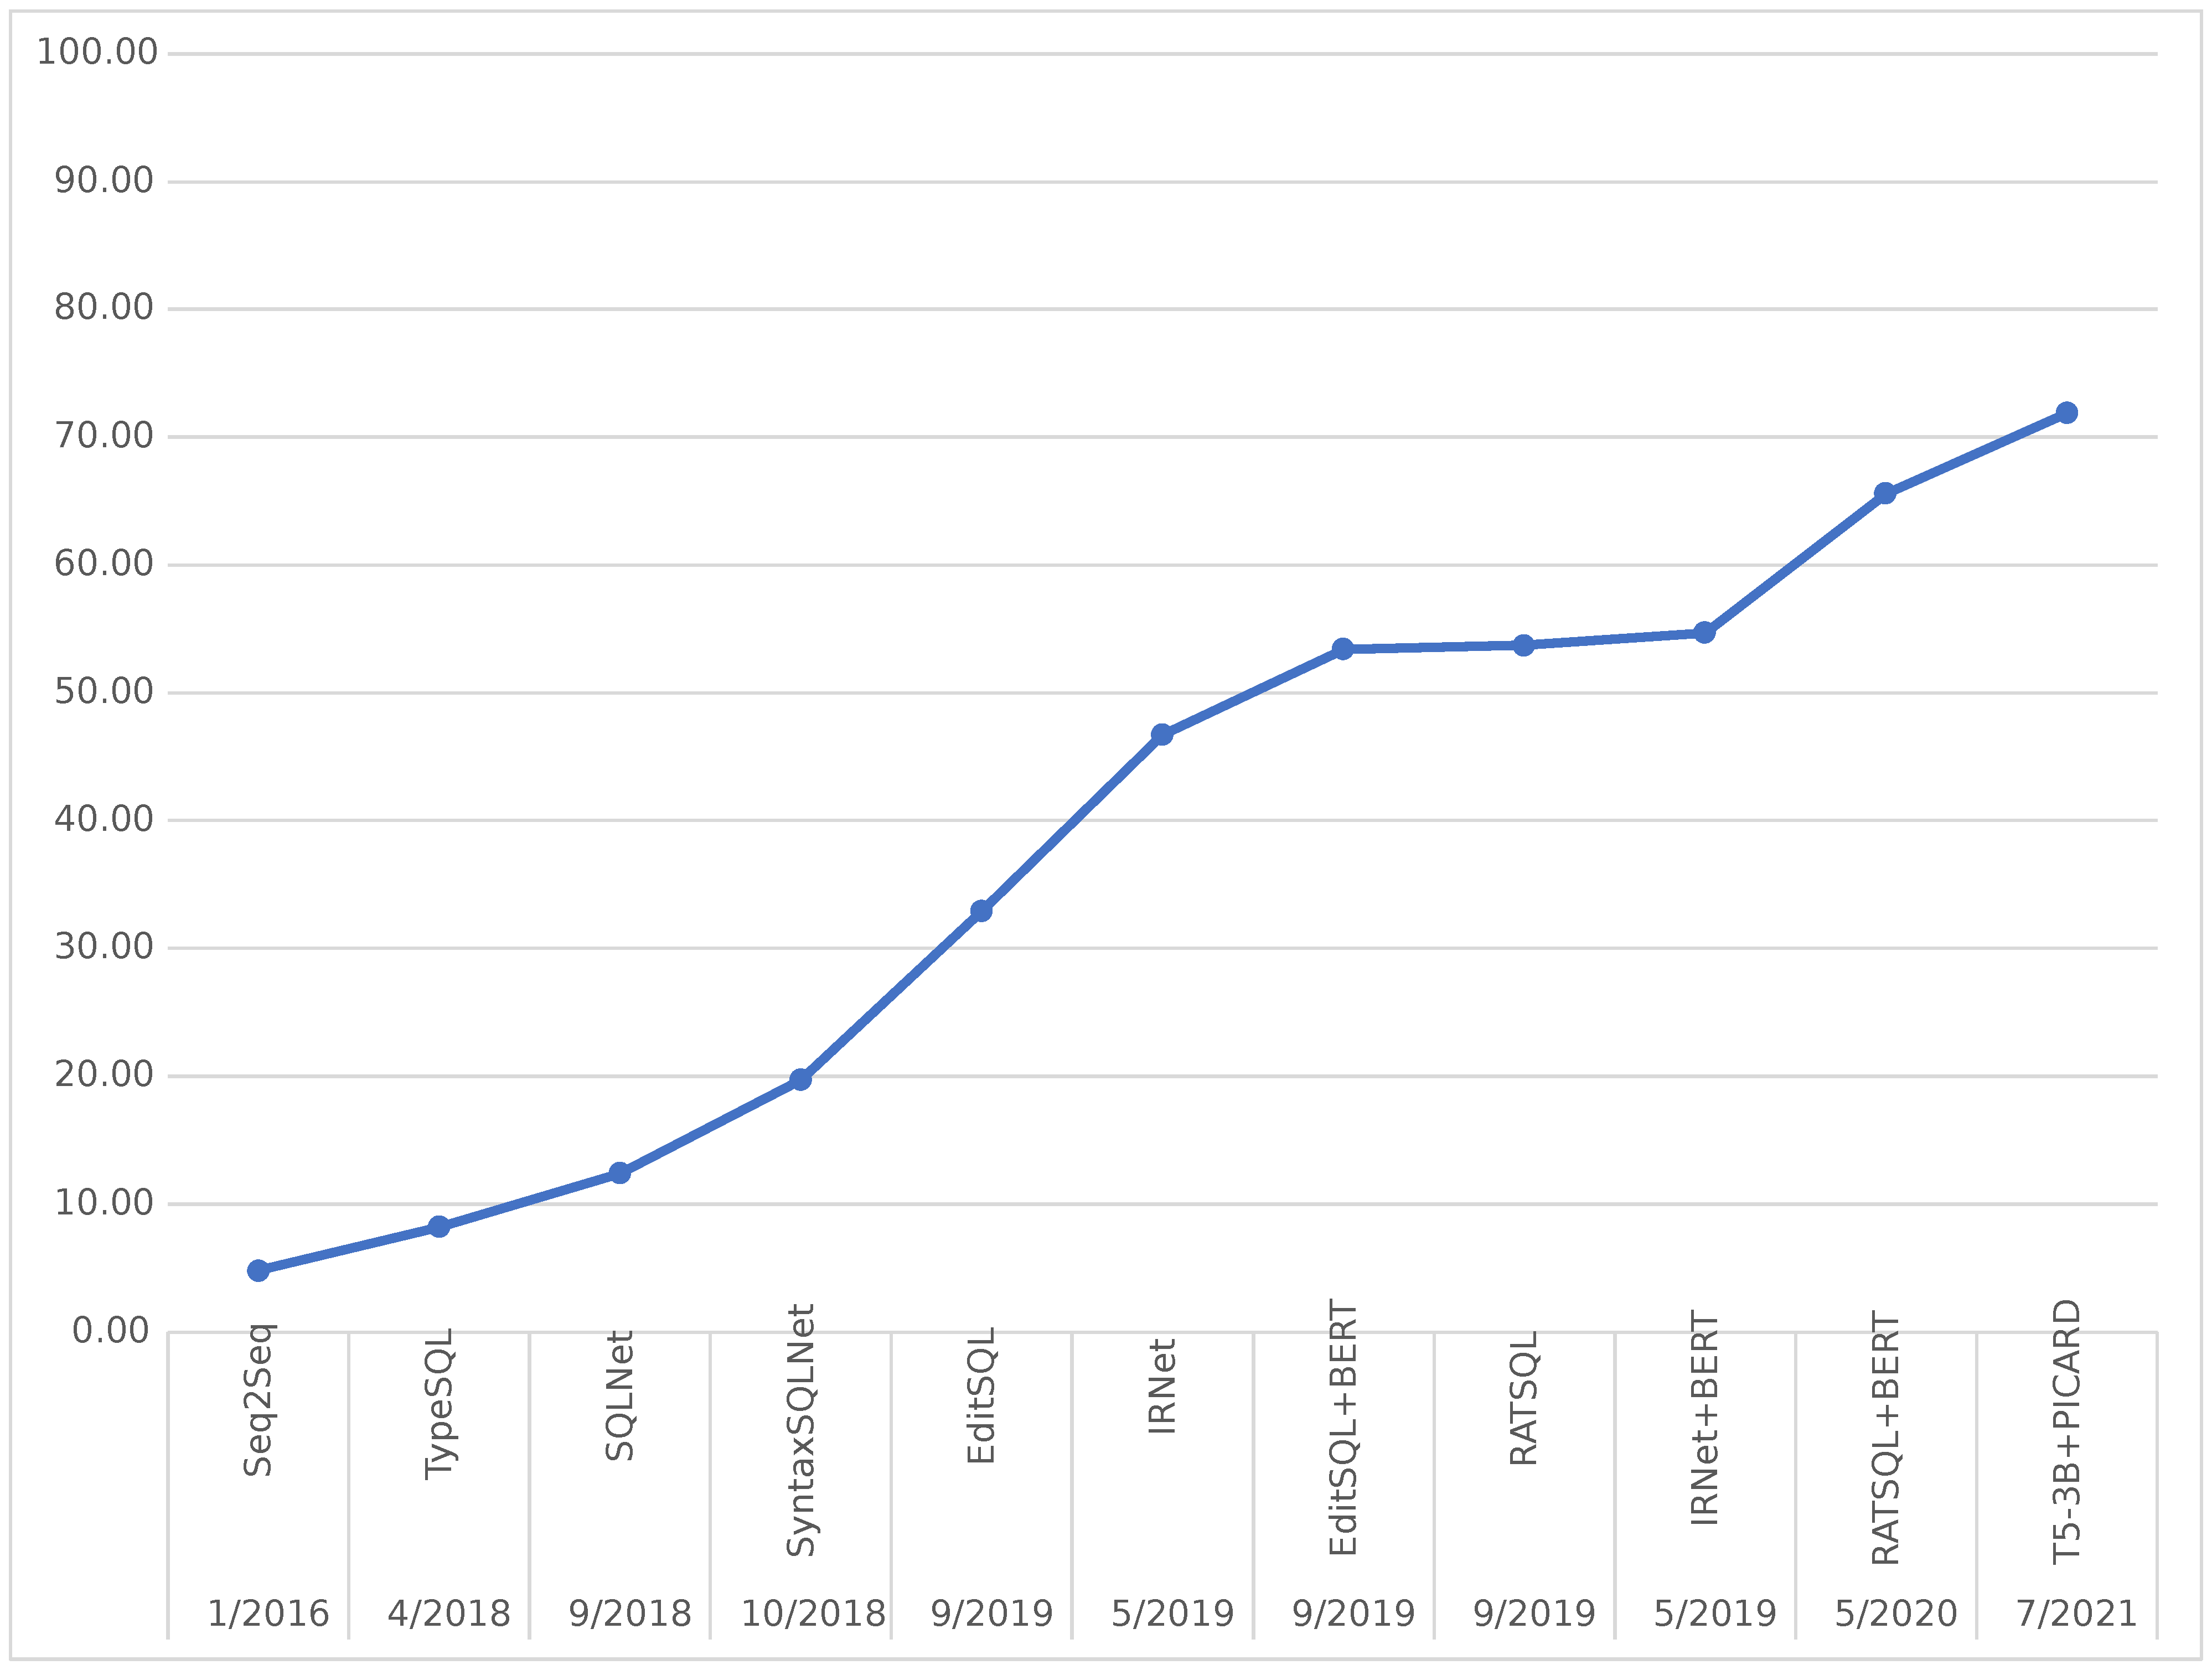
\includegraphics[width=0.99\linewidth]{pics/benchmarkeps}
    \caption{SPIDER benchmark Exact Match Results including our experiments}
    \label{fig:benchmark}
\end{figure}
\clearpage
\subsection{EZ-PICARD - Microservices Practices}

% add image here
\begin{figure}[h]
    \centering
    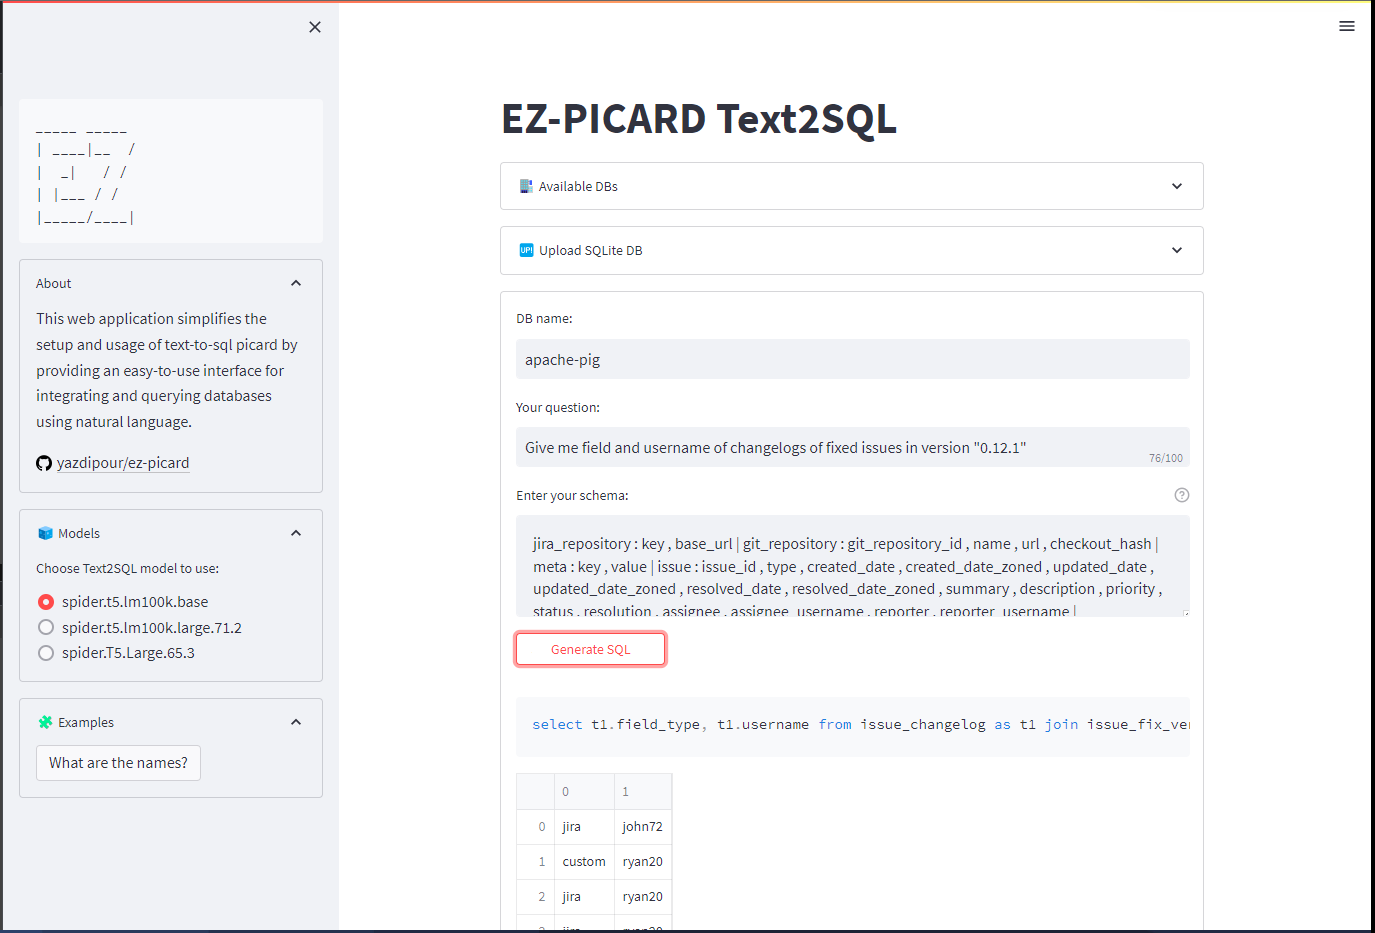
\includegraphics[width=1\textwidth]{pics/ez/ui.png}
    \caption{EZ-PICARD Web Application}
    \label{fig:ezpicard}
\end{figure}

For software engineering practices and to make PICARD setup easier for engineers, researchers, and users, a microservice web service with a web application has been created and open-sourced to the community\footnote[1]{Link to the Github Page: \url{https://github.com/yazdipour/ez-picard/}}. This application consists of a web user interface that gives users the ability to upload their databases and enter their natural language questions and receive queries from our model with values from the database if available. Additionally, a REST API exists for further expansion and usage within the application, providing users with a more versatile and powerful tool for their needs. This web service and application is designed to make the usage of PICARD easier and more accessible for everyone and to allow for the development of new applications and services that utilize its powerful capabilities.

PICARD is a method for constrained inference on top of an existing model, but it is not a model itself. Currently, the PICARD parser and the supporting software are not supported for PostgreSQL, MySQL and others, which would require changes to the PICARD parser, translation of Spider databases and text-to-SQL data, and retraining models to produce MSSQL code. To use the Picard Method, a complex toolchain of Haskell code is built with CABAL and requires a complicated toolchain for the Facebook Thrift library.

% After the setup, the Picard server can be started by running the compiled standalone executable PICARD. This executable is responsible for providing the necessary information to the user, such as specific parameters and options within the constrained inference.

The thrift library is used for communication between the parser and the beam search algorithm. The parser, written in the efficient and powerful Haskell programming language, is used in combination with the hf transformers, which is a Python package. To further expand the scope of the system, new SQL engines can be supported by adding a parser for each one.

These parsers also need to be written in Haskell, as the existing SQLite parser is of limited use in this regard, as it has been written to work best on Spider's subset of SQLite and only supports part of the SQLite specification. This means that more advanced parsers must be created to maximize the system's capabilities. Additionally, these parsers need to be written with a high level of precision in order to ensure that the system can effectively communicate with various engines and databases.

With EZ-PICARD, we can have an adapter layer between SQLite DB and any other database engine, such as MySQL. This layer can be implemented independently from PICARD itself using Python instead of Haskell and can provide a wide range of features, such as automatically translating queries from SQLite to the target database engine and mirroring the schema to the SQLite DB. This adapter layer can provide further advantages by allowing developers to use the same codebase to support multiple database engines, thus reducing the need for additional development and maintenance costs.

% add image here
\begin{figure}[h]
    \centering
    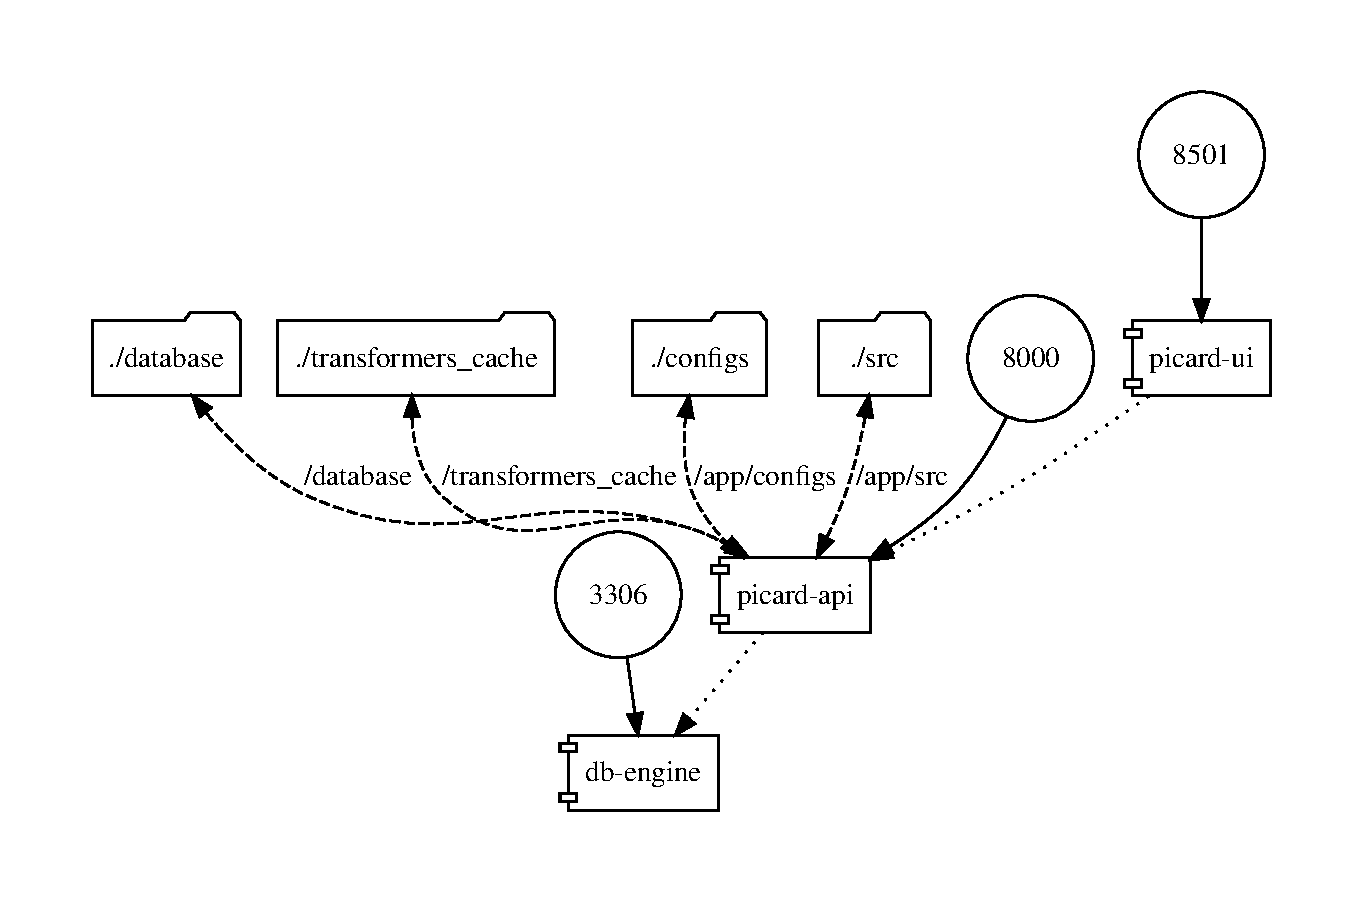
\includegraphics[width=0.8\textwidth]{pics/ez/mapeps}
    \caption{EZ-PICARD Architecture}
\end{figure}